%!TEX root = ../thesis_master.tex
%*******************************************************************************
% * Copyright (c) 2006-2013 
% * Institute of Automation, Dresden University of Technology
% * 
% * All rights reserved. This program and the accompanying materials
% * are made available under the terms of the Eclipse Public License v1.0 
% * which accompanies this distribution, and is available at
% * http://www.eclipse.org/legal/epl-v10.html
% * 
% * Contributors:
% *   Institute of Automation - TU Dresden, Germany 
% *      - initial API and implementation
% ******************************************************************************/

When dealing with object manipulation, it is necessary that the robot adopts a certain pose with respect to the target before the proper manipulation process starts. In this thesis, an \emph{Image Based Visual Servoing} (IBVS) controller for the translational and yaw kinematics of an aerial robot is designed and implemented. 

Using only image data, the controller computes the necessary robot's velocities to achieve the desired pose with respect to a planar object laying on the ground. To this end, some visual features are calculated from the current and desired poses and their difference is used as error by a PID controller that outputs the velocity commands sent to the vehicle's low-level controllers.

The controller is implemented as a ROS component, so it can be integrated part of a modular robotic system running on this framework. Finally, the system is tested and verified in a simulation of a quadrotor aerial robot.

\begin{center}
	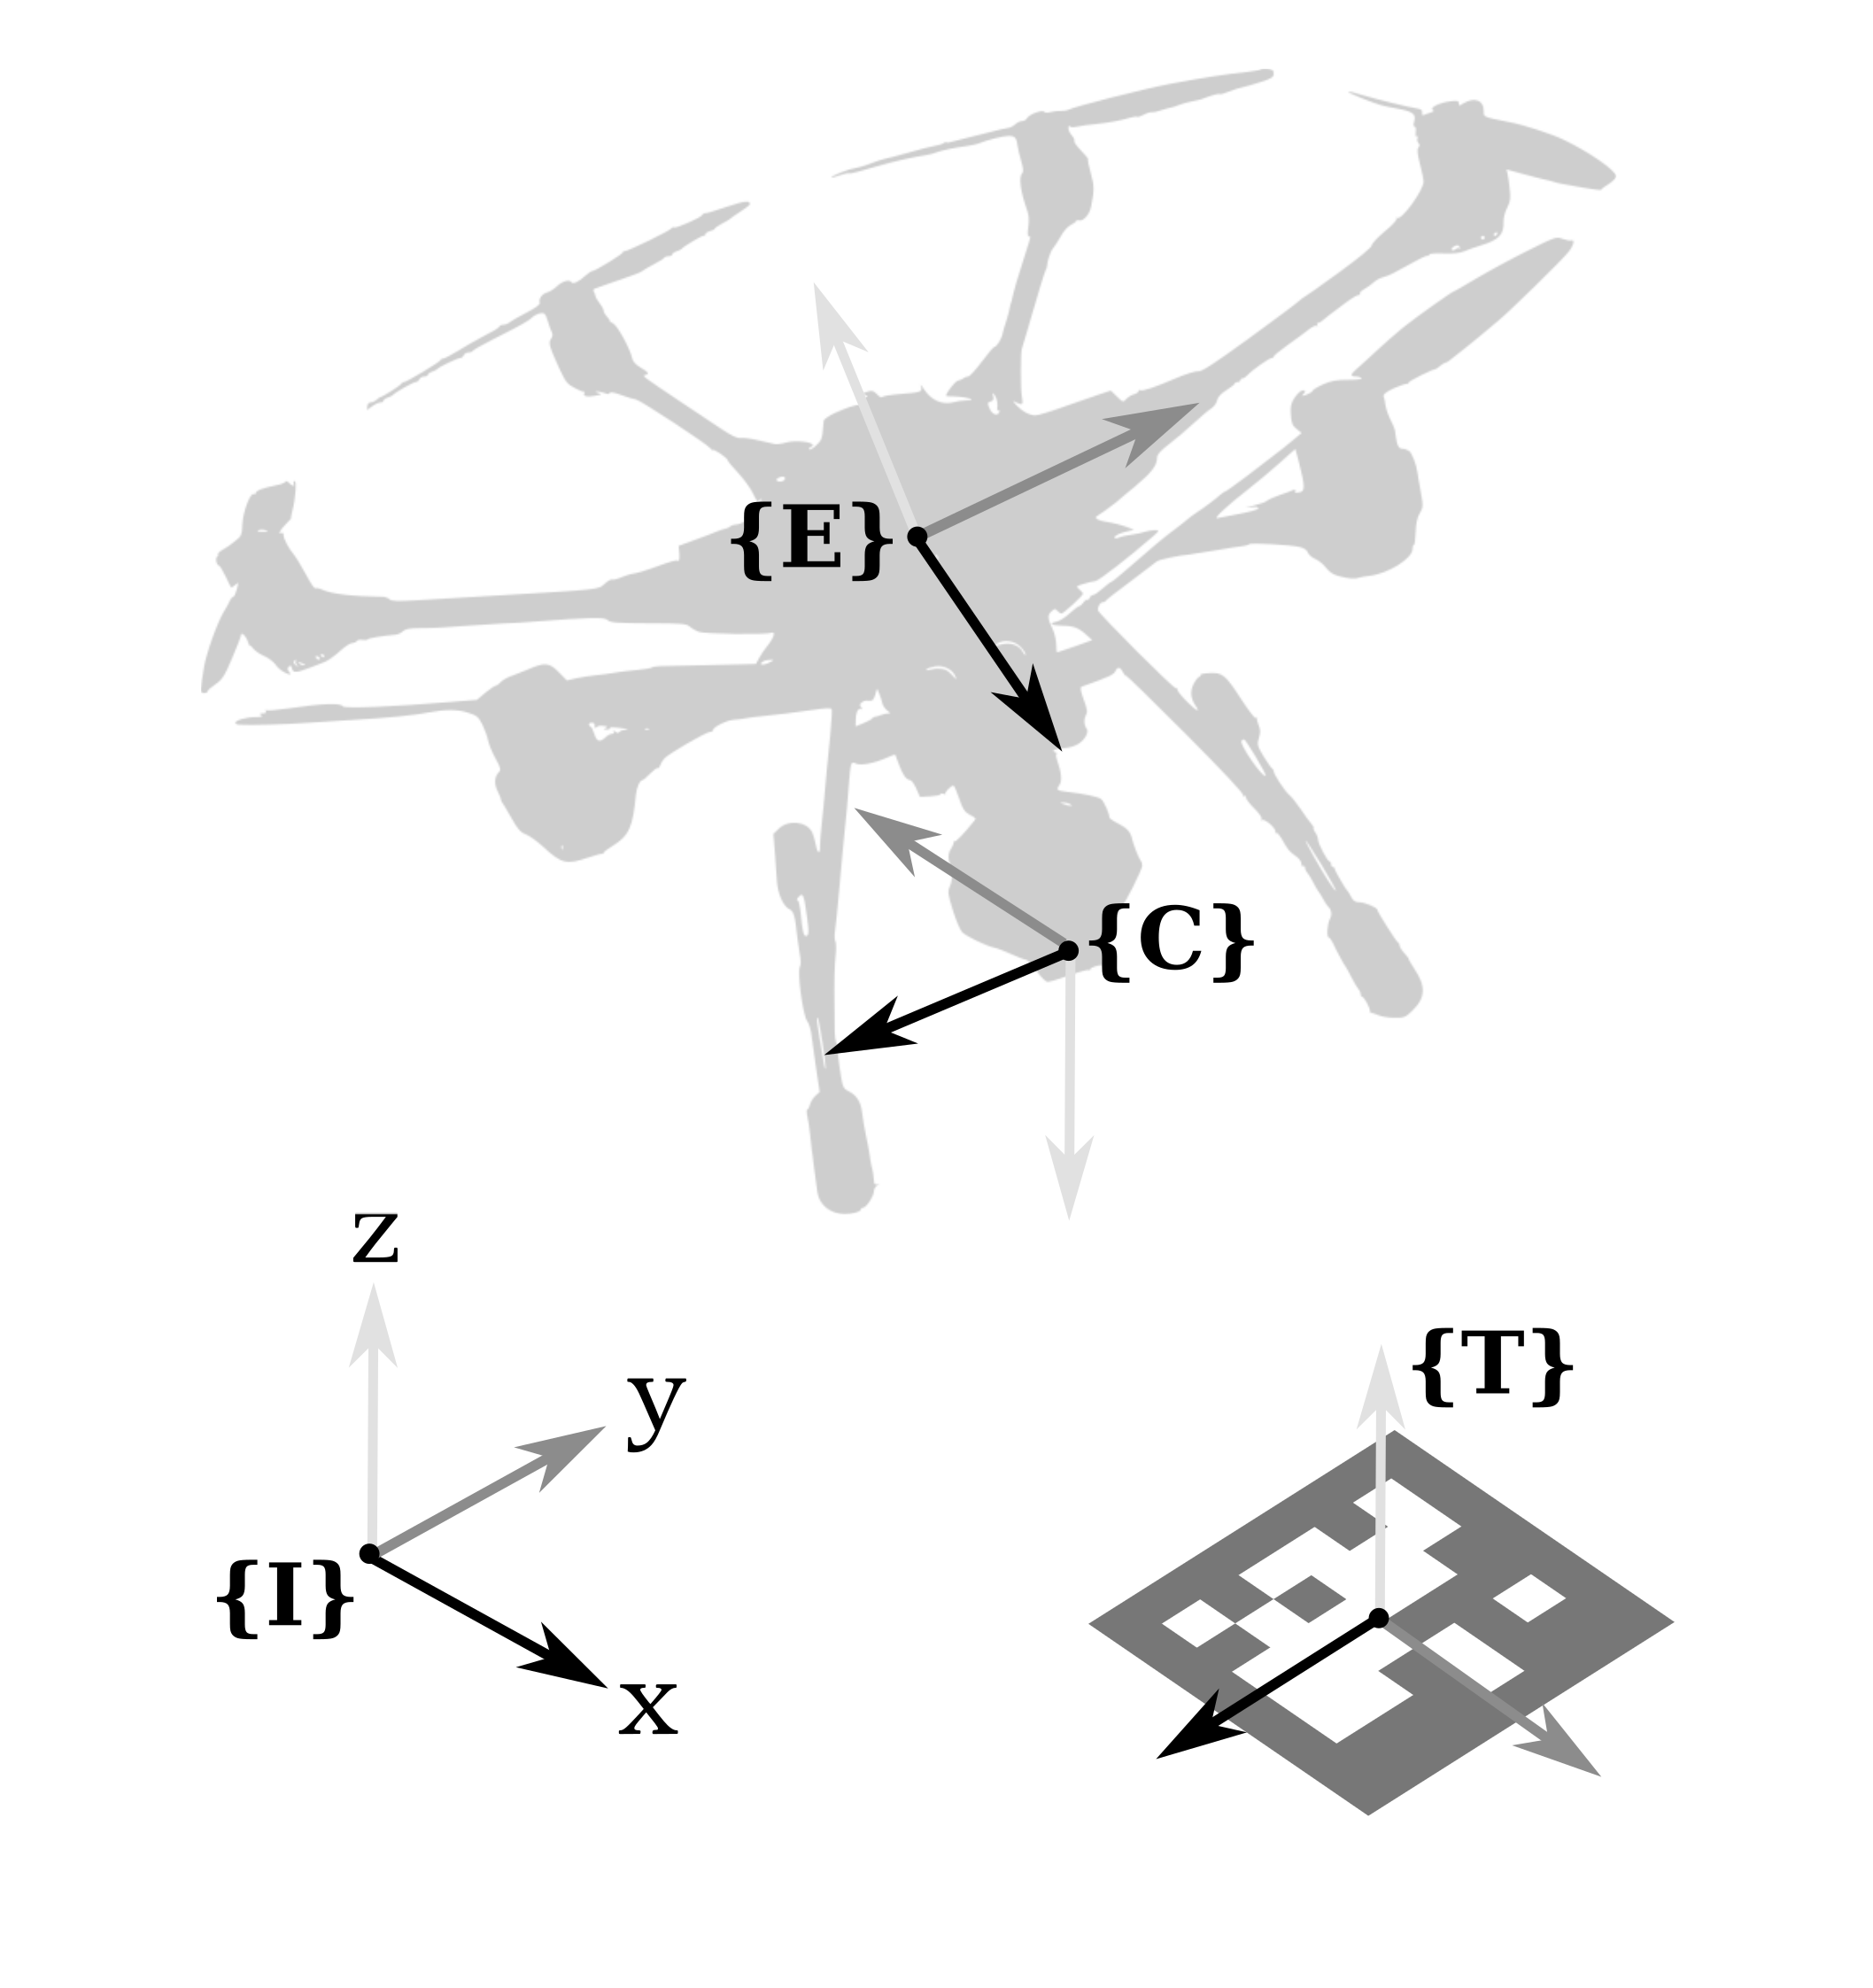
\includegraphics[keepaspectratio, width=6.5cm]{content/frames_bw.png}
\end{center}